% !TeX program = xelatex
\documentclass[a4paper,10pt]{article}

% ============================================================================
% សន្លឹកកិច្ចការសិស្ស ស-ខ្មៅ (Student Fill-In Worksheet — No-LCD Classroom)
% មេរៀនទី១៧ (១៧.៤)៖ ការគណនាមាឌនៃកោន និងលំហាត់សំយោគ (ត្រូវគ្នា ១០០% នឹង LS_Plan_CONE_VOL.tex)
% ============================================================================
\usepackage[a4paper, left=0.95cm, right=0.95cm, top=0.75cm, bottom=0.90cm, footskip=0.48cm]{geometry}
\usepackage{amsmath}
\usepackage{unicode-math}
\usepackage{fontspec}
\usepackage{array, colortbl}
\usepackage[table]{xcolor}
\usepackage{enumitem}
\usepackage{pifont}
\usepackage{fancyhdr}
\usepackage{lastpage}
\usepackage{tikz}
\usepackage[most]{tcolorbox}
\usetikzlibrary{calc, arrows.meta, angles, quotes, patterns, decorations.markings, babel}

\makeatletter
\let\@expl@@@mark@update@singlecol@structures@@\relax
\makeatother

\providecommand{\NGSFindFonts}{%
  \IfFileExists{C:/Windows/Fonts/cambria.ttc}{%
    \def\NGSSysPath{C:/Windows/Fonts/}%
    \def\NGSUserPath{C:/Users/KIT/AppData/Local/Microsoft/Windows/Fonts/}%
  }{%
    \IfFileExists{./fonts/KhmerOSsiemreap.ttf}{\def\NGSSysPath{./fonts/}\def\NGSUserPath{./fonts/}}{%
    \IfFileExists{../fonts/KhmerOSsiemreap.ttf}{\def\NGSSysPath{../fonts/}\def\NGSUserPath{../fonts/}}{%
    \IfFileExists{../../fonts/KhmerOSsiemreap.ttf}{\def\NGSSysPath{../../fonts/}\def\NGSUserPath{../../fonts/}}{%
    \IfFileExists{../../../fonts/KhmerOSsiemreap.ttf}{\def\NGSSysPath{../../../fonts/}\def\NGSUserPath{../../../fonts/}}{%
    \IfFileExists{../../../../fonts/KhmerOSsiemreap.ttf}{\def\NGSSysPath{../../../../fonts/}\def\NGSUserPath{../../../../fonts/}}{%
    \IfFileExists{../../../../../fonts/KhmerOSsiemreap.ttf}{\def\NGSSysPath{../../../../../fonts/}\def\NGSUserPath{../../../../../fonts/}}{%
    \IfFileExists{../../../../../../fonts/KhmerOSsiemreap.ttf}{\def\NGSSysPath{../../../../../../fonts/}\def\NGSUserPath{../../../../../../fonts/}}{%
      \def\NGSSysPath{../../../../../../../fonts/}\def\NGSUserPath{../../../../../../../fonts/}%
    }}}}}}}%
  }%
}
\NGSFindFonts

\setmathfont[Path={\NGSSysPath}, FontIndex=1, Scale=1.02]{cambria.ttc}
\defaultfontfeatures{Ligatures=TeX}

\setmainfont[
  Path={\NGSUserPath},
  Extension=.ttf,
  Script=Khmer,
  BoldFont={KhmerOSsiemreap},
  BoldFeatures={FakeBold=1.8},
  ItalicFont={KhmerOSsiemreap},
  ItalicFeatures={FakeSlant=0.25},
  BoldItalicFont={KhmerOSsiemreap},
  BoldItalicFeatures={FakeBold=1.8, FakeSlant=0.25}
]{KhmerOSsiemreap}

\newfontfamily\muol[Path={\NGSUserPath}, Extension=.ttf, Script=Khmer]{KhmerOSmuollight}
\newfontfamily\TimesEn[Path={\NGSSysPath}, Extension=.ttf, BoldFont={timesbd}, ItalicFont={timesi}, BoldItalicFont={timesbi}]{times}

\XeTeXlinebreaklocale "km"
\XeTeXlinebreakskip = 0pt plus 1pt minus 0.1pt

\definecolor{panelgray}{gray}{0.93}
\definecolor{headgray}{gray}{0.85}

\pagestyle{fancy}
\fancyhf{}
\renewcommand{\headrulewidth}{0pt}
\fancyfoot[L]{\fontsize{8pt}{10pt}\selectfont អនុវិទ្យាល័យព្រះក្រសាំង \en{---} គណិតវិទ្យា ថ្នាក់ទី៨ \en{|} មេរៀនទី១៧ (១៧.៤ ការគណនាមាឌនៃកោន និងលំហាត់សំយោគ)}
\fancyfoot[R]{\fontsize{8.2pt}{10pt}\selectfont ទំព័រ \en{\thepage\ / \pageref{LastPage}}}

\setlength{\parindent}{0pt}
\setlength{\parskip}{0pt}
\setlength{\tabcolsep}{4pt}

\newcommand{\en}[1]{{\TimesEn #1}}
\newcommand{\enbf}[1]{{\TimesEn\textbf{#1}}}
\newcommand{\unit}[1]{\,\text{\en{#1}}}
\newcommand{\cnum}[1]{\mbox{\fontsize{10pt}{12pt}\selectfont\ding{\numexpr181+#1\relax}}}
\newcommand{\chkbox}{\tikz[baseline=-0.15ex]\draw[black, line width=0.85pt] (0,0) rectangle (0.25cm,0.25cm);}
\newcommand{\blank}[1]{\makebox[#1]{\dotfill}}
\newcommand{\tri}[1]{\ensuremath{\triangle #1}}

\newcommand{\rightbox}[4][0.18]{%
  \draw[black, line width=0.8pt]
    ($(#3)!#1!(#2)$) -- ($($(#3)!#1!(#2)$)+($(#3)!#1!(#4)$)-(#3)$) -- ($(#3)!#1!(#4)$);
}

\newcommand{\secbar}[2]{%
  \vspace{3pt}%
  \begin{tcolorbox}[
    enhanced, sharp corners, colback=headgray, colframe=black,
    boxrule=0.9pt, boxsep=1pt, top=2.5pt, bottom=2.5pt, left=6pt, right=6pt,
    after skip=3pt
  ]
    {\muol\fontsize{9.2pt}{13.5pt}\selectfont #1}\hfill{\fontsize{8.3pt}{11.5pt}\selectfont\textbf{#2}}
  \end{tcolorbox}%
}

\newcolumntype{L}[1]{>{\raggedright\arraybackslash}p{#1}}
\newcolumntype{C}[1]{>{\centering\arraybackslash}p{#1}}

\begin{document}
\fontsize{9.4pt}{13.8pt}\selectfont

% ============================================================================
% ទំព័រទី ១៖ ក្បាលសន្លឹកកិច្ចការ + E1 (អណ្ដូងទឹកទី១៨) + E2 (សមាមាត្រ 1/3 & វិភាគកំហុស s vs h) + E3 (សំយោគសូលីត ៤)
% ============================================================================
\begin{tcolorbox}[
  enhanced, sharp corners, colback=white, colframe=black,
  boxrule=1.1pt, boxsep=2.5pt, top=6pt, bottom=6pt, left=6pt, right=6pt, after skip=8pt
]
  \begin{center}
    {\muol\fontsize{10pt}{14.5pt}\selectfont សន្លឹកកិច្ចការសិស្ស \enbf{---} គណិតវិទ្យា ថ្នាក់ទី៨ \enbf{(}១៧\enbf{.}៤ មាឌនៃកោន និងសំយោគមេរៀនទី១៧\enbf{)}}\\[3.5pt]
    {\fontsize{8.8pt}{12pt}\selectfont
    ឈ្មោះសិស្ស / ដៃគូ៖ \blank{6.2cm} \hspace{0.2cm}
    ថ្នាក់៖ \blank{1.4cm} \hspace{0.2cm}
    ក្រុម៖ \blank{1.2cm} \hspace{0.2cm}
    កាលបរិច្ឆេទ៖ \blank{2.8cm}}
  \end{center}
\end{tcolorbox}

% --- E1 Engage: Water Well Engineering Mystery (Ex #18 p. 229) ---
\begin{tcolorbox}[
  enhanced, sharp corners, colback=panelgray, colframe=black,
  boxrule=0.8pt, boxsep=2.5pt, top=6pt, bottom=6pt, left=6pt, right=6pt, after skip=8pt
]
  \textbf{បេសកកម្មទី១ (\en{E1 - Engage / POE})៖ គណនាចំណុះបាតអណ្ដូងទឹករាងកោន (លំហាត់ទី១៨ ទំព័រ ២២៩)}\\[3pt]
  គេជីកអណ្ដូងទឹកមួយមានតួលើរាងស៊ីឡាំងអង្កត់ផ្ចិតមាត់ $d = 6\unit{m}$ ($r=3\unit{m}$) ជម្រៅ $50\unit{m}$ និងបាតក្រោមរាងកោនដែលមានជនេត្រទ្រេត $s = 5\unit{m}$ ។ មុនពេលគណនាមាឌអណ្ដូងទាំងមូល ចូរទស្សន៍ទាយមាឌផ្នែកបាតរាងកោនខាងក្រោម៖\\[3pt]
  \ding{226}\ ទស្សន៍ទាយជាដៃគូមុនរៀន៖ \;\chkbox\ $15\pi\unit{m}^3$ \hspace{1.1cm} \chkbox\ $12\pi\unit{m}^3$ \hspace{1.1cm} \chkbox\ $36\pi\unit{m}^3$
\end{tcolorbox}

% --- E2 Explore Part A: 3-to-1 Cylinder-vs-Cone & Worked Example 1 (p. 225) ---
\secbar{ផ្នែកទី១ \enbf{(}ក\enbf{)} ៖ ការប្រៀបធៀបស៊ីឡាំង\enbf{-}កោន និងលំហាត់គំរូទី \enbf{1 (}ទំព័រ ២២៥\enbf{) (E2 - Explore)}}{ការងារជាដៃគូ \en{5 min}}

\noindent
\begin{minipage}[c]{7.8cm}
  \centering
  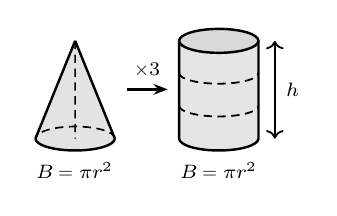
\begin{tikzpicture}[scale=0.80, every node/.style={font=\scriptsize, text=black}]
    % កោន x 3 = ស៊ីឡាំង
    \coordinate (V) at (-1.35,0.85);
    \coordinate (L) at (-1.98,-0.70);
    \coordinate (R) at (-0.72,-0.70);
    \fill[gray!22] (L) -- (V) -- (R) arc (0:-180:0.63 and 0.19);
    \draw[black, line width=0.88pt] (L) arc (-180:0:0.63 and 0.19) (V) -- (L) (V) -- (R);
    \draw[black, line width=0.6pt, densely dashed] (R) arc (0:180:0.63 and 0.19) (V) -- (-1.35,-0.70);
    \node[below=1pt] at (-1.35,-0.88) {$B=\pi r^2$};

    \draw[-{Stealth[length=1.8mm]}, line width=0.85pt] (-0.52,0.08) -- (0.12,0.08) node[midway, above=1pt] {$\times 3$};

    \fill[gray!20] (0.30,-0.70) -- (0.30,0.85) arc (180:360:0.63 and 0.19) -- (1.56,-0.70) arc (0:-180:0.63 and 0.19);
    \fill[gray!30] (0.93,0.85) ellipse (0.63 and 0.19);
    \draw[black, line width=0.65pt, densely dashed] (0.30,-0.18) arc (-180:0:0.63 and 0.17) (0.30,0.34) arc (-180:0:0.63 and 0.17);
    \draw[black, line width=0.88pt] (0.93,0.85) ellipse (0.63 and 0.19);
    \draw[black, line width=0.88pt] (0.30,-0.70) -- (0.30,0.85) (1.56,-0.70) -- (1.56,0.85) (0.30,-0.70) arc (-180:0:0.63 and 0.19);
    \draw[<->, line width=0.65pt] (1.82,-0.70) -- (1.82,0.85) node[midway, right=0.5pt] {$h$};
    \node[below=1pt] at (0.93,-0.88) {$B=\pi r^2$};
  \end{tikzpicture}
\end{minipage}%
\hfill
\begin{minipage}[c]{10.8cm}\raggedright
  \textbf{ពិនិត្យដ្យាក្រាមទំ.២២៥ និងអនុវត្តលំហាត់គំរូទី \en{1} ($\pi\approx 3.14$)៖}\\[5.5pt]
  $1.$ កោននិងស៊ីឡាំងមានបាតថាសកាំ $r$ ($B = \pi r^2$) និងកម្ពស់កែង $h$ ស្មើគ្នា៖\\
  \hspace*{0.3cm}ចាក់ខ្សាច់ពេញកោនចូលក្នុងស៊ីឡាំង \blank{0.8cm} ដង ទើបពេញស៊ីឡាំង\\[4pt]
  \hspace*{0.3cm}$\Rightarrow V_{\text{កោន}} = \dfrac{1}{\blank{0.7cm}} B \cdot h = \dfrac{1}{\blank{0.7cm}} \pi \times \blank{0.8cm} \times \blank{0.8cm}$ ។\\[5.5pt]
  $2.$ \textbf{គំរូទី \en{1} (ទំ.២២៥)៖} កោនមានកាំបាត $r = 3\unit{m}$ និងកម្ពស់កែង $h = 8\unit{m}$៖\\[4pt]
  \hspace*{0.3cm}$V = \dfrac{1}{3}\times 3.14\times (\blank{0.7cm})^2\times 8 = 3.14\times \blank{0.9cm} = \blank{1.4cm}\unit{m}^3$ ។
\end{minipage}

\vspace{23pt}
% --- E2 Explore Part B: Error-Analysis on Worked Example 2 (p. 226) ---
\secbar{ផ្នែកទី១ \enbf{(}ខ\enbf{)} ៖ វិភាគកំហុស \enbf{«}សិស្ស ក ទល់ សិស្ស ខ\enbf{»} លើគំរូទី \enbf{2 (}ទំព័រ ២២៦ \enbf{---} $s$ ទល់ $h$\enbf{)}}{ការងារជាដៃគូ \en{6 min}}

\begin{tcolorbox}[
  enhanced, sharp corners, colback=white, colframe=black,
  boxrule=0.8pt, boxsep=3.5pt, top=8pt, bottom=8pt, left=5.5pt, right=5.5pt
]
  \begin{minipage}[c]{3.2cm}
    \centering
    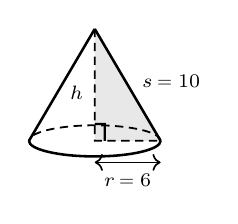
\begin{tikzpicture}[scale=0.76, every node/.style={font=\scriptsize, text=black}]
      \coordinate (V) at (0,1.15);
      \coordinate (O) at (0,-0.72);
      \coordinate (L) at (-1.10,-0.72);
      \coordinate (R) at (1.10,-0.72);
      \fill[gray!18] (V) -- (O) -- (R) -- cycle;
      \draw[black, line width=0.92pt] (L) arc (-180:0:1.10 and 0.26) (V) -- (L) (V) -- (R);
      \draw[black, line width=0.65pt, densely dashed] (R) arc (0:180:1.10 and 0.26) (V) -- (O) -- (R);
      \rightbox[0.15]{V}{O}{R}
      \node[left=0.5pt] at (0,0.08) {$h$};
      \draw[<->, line width=0.6pt] (0,-1.08) -- (1.10,-1.08) node[midway, below=0.5pt] {$r=6$};
      \node[right=1pt] at (0.58,0.28) {$s=10$};
    \end{tikzpicture}
  \end{minipage}%
  \hfill
  \begin{minipage}[c]{14.5cm}\raggedright
    \textbf{ប្រធានគំរូទី \en{2} (ទំ.២២៦)៖} គណនាមាឌកោនដែលមានកាំបាត $r = 6$ និងជនេត្រ $s = 10$ ($\pi\approx 3.14$) ។\\[5.5pt]
    $\bullet$ \textbf{ដំណោះស្រាយសិស្ស ក៖} $V = \dfrac{1}{3}\times 3.14\times 6^2\times 10 = 376.8$ \hspace{0.35cm} (\chkbox\ ត្រូវ \;/\; \chkbox\ ខុស)\\[5.5pt]
    $\bullet$ \textbf{ដំណោះស្រាយសិស្ស ខ៖} រកកម្ពស់កែងតាមពីតាករសិន៖ $h = \sqrt{10^2 - 6^2} = \sqrt{\blank{0.9cm}} = \blank{0.8cm}$\\[4.5pt]
    \hspace*{0.25cm}រួចគណនាមាឌ៖ $V = \dfrac{1}{3}\times 3.14\times 6^2\times \blank{0.8cm} = \blank{1.3cm} \approx \blank{1.2cm}$ ឯកតាមាឌ \; (\chkbox\ ត្រូវ \;/\; \chkbox\ ខុស)\\[5.5pt]
    $\bullet$ \textbf{សន្និដ្ឋាន៖} សិស្ស ក ខុសព្រោះបានយក \blank{2.2cm} ជំនួសឱ្យកម្ពស់កែង $h$!
  \end{minipage}
\end{tcolorbox}

\vspace{23pt}
% --- E3 Explain: Complete Lesson 17 Synthesis Table (All 4 Solids + Reverse Formula) ---
\secbar{ផ្នែកទី២ ៖ សំយោគរូបមន្តសូលីតទាំង ៤ នៃមេរៀនទី១៧ និងការទាញបញ្ច្រាសរូបមន្ត \enbf{(E3 - Explain)}}{សង្ខេបរួមគ្នា \en{6 min}}

\begin{tcolorbox}[
  enhanced, sharp corners, colback=white, colframe=black,
  boxrule=0.9pt, boxsep=4.5pt, top=10pt, bottom=10pt, left=6pt, right=6pt
]
  {\renewcommand{\arraystretch}{2.12}\footnotesize
  \begin{tabular}{|L{4.25cm}|L{3.95cm}|L{4.10cm}|L{4.65cm}|}
    \hline
    \cellcolor{headgray}\textbf{ប្រភេទសូលីត (មេរៀនទី១៧)} & \cellcolor{headgray}\textbf{ផ្ទៃក្រឡាខាង ($S_l$)} & \cellcolor{headgray}\textbf{ផ្ទៃទាំងអស់ ($S_T$)} & \cellcolor{headgray}\textbf{រូបមន្តមាឌ ($V$)} \\
    \hline
    $1.$ ព្រីសត្រង់ និង ស៊ីឡាំង & $P\cdot h$ \;\textbar\; $2\pi r h$ & $S_l + 2B$ & $V = B\cdot h$ \;\textbar\; $\pi r^2 h$ \\
    \hline
    $2.$ ពីរ៉ាមីតនិយ័ត & $\dfrac{1}{2} P \cdot d$ & $S_l + B$ & $V = \dfrac{1}{3} B \cdot h$ ($h$ កែងបាត) \\
    \hline
    $3.$ កោនបរិវត្ត (កាំ $r$, ជនេត្រ $s$) & $\pi r s$ & $\pi r s + \pi r^2$ & $V = \dfrac{1}{\blank{0.7cm}} \pi r^2 \blank{0.7cm}$ ($h=\sqrt{s^2-r^2}$) \\
    \hline
  \end{tabular}}\\[9pt]
  $\bullet$ \textbf{ការទាញបញ្ច្រាសរូបមន្តកោន/ពីរ៉ាមីត៖} ពី $V = \dfrac{1}{3}B\cdot h \Rightarrow h = \dfrac{\blank{0.7cm} V}{B}$ \;\text{និង}\; $B = \dfrac{\blank{0.7cm} V}{h}$\\[6.5pt]
  $\bullet$ \textbf{ធនាគារហេតុផល៖}
  \cnum{1} $B = \pi r^2$ \;\textbar\;
  \cnum{2} $h = \sqrt{s^2-r^2}$ ឬ $r = \sqrt{s^2-h^2}$ \;\textbar\;
  \cnum{3} $V = \dfrac{1}{3}\pi r^2 h$ \;\textbar\;
  \cnum{4} $B = \dfrac{3V}{h},\; h = \dfrac{3V}{B}$
\end{tcolorbox}

\newpage

% ============================================================================
% ទំព័រទី ២៖ E4 (ប្រតិបត្តិ ក,ខ ទំ.២២៦ & ទី១៣ ទំ.២២៩) + E5 (អណ្ដូងទឹកទី១៨ & Exit Check) + កិច្ចការផ្ទះ
% ============================================================================

\secbar{ផ្នែកទី៣ ៖ អនុវត្តលំហាត់ប្រតិបត្តិទំព័រ ២២៦ និងលំហាត់សំយោគទី១៣ \enbf{(E4 - Elaborate)}}{អនុវត្ត \en{10 min}}

\noindent
\begin{minipage}[t]{9.6cm}\vspace{0pt}
  \begin{tcolorbox}[
    enhanced, sharp corners, colback=white, colframe=black, equal height group=rowE4,
    boxrule=0.85pt, boxsep=3.5pt, top=7pt, bottom=7pt, left=5.5pt, right=5.5pt
  ]\raggedright
    \textbf{៣.ក ប្រតិបត្តិ ក និង ខ (ទំ.២២៦, $\pi\approx 3.14$)៖}
    \begin{center}
      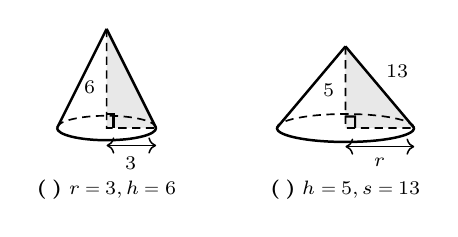
\begin{tikzpicture}[scale=0.74, every node/.style={font=\scriptsize, text=black}]
        % (ក) r=3, h=6
        \begin{scope}[shift={(-2.05,0)}]
          \coordinate (V) at (0,1.08);
          \coordinate (O) at (0,-0.62);
          \coordinate (L) at (-0.85,-0.62);
          \coordinate (R) at (0.85,-0.62);
          \fill[gray!18] (V) -- (O) -- (R) -- cycle;
          \draw[black, line width=0.9pt] (L) arc (-180:0:0.85 and 0.21) (V) -- (L) (V) -- (R);
          \draw[black, line width=0.6pt, densely dashed] (R) arc (0:180:0.85 and 0.21) (V) -- (O) -- (R);
          \rightbox[0.14]{V}{O}{R}
          \node[left=0.5pt] at (0,0.08) {$6$};
          \draw[<->, line width=0.55pt] (0,-0.92) -- (0.85,-0.92) node[midway, below=0.5pt] {$3$};
          \node at (0,-1.68) {\textbf{(ក)} $r=3, h=6$};
        \end{scope}
        % (ខ) h=5, s=13
        \begin{scope}[shift={(2.05,0)}]
          \coordinate (V) at (0,0.78);
          \coordinate (O) at (0,-0.62);
          \coordinate (L) at (-1.18,-0.62);
          \coordinate (R) at (1.18,-0.62);
          \fill[gray!18] (V) -- (O) -- (R) -- cycle;
          \draw[black, line width=0.9pt] (L) arc (-180:0:1.18 and 0.24) (V) -- (L) (V) -- (R);
          \draw[black, line width=0.6pt, densely dashed] (R) arc (0:180:1.18 and 0.24) (V) -- (O) -- (R);
          \rightbox[0.14]{V}{O}{R}
          \node[left=0.5pt] at (0,0.02) {$5$};
          \draw[<->, line width=0.55pt] (0,-0.94) -- (1.18,-0.94) node[midway, below=0.5pt] {$r$};
          \node[above right=-1pt] at (0.58,0.12) {$13$};
          \node at (0,-1.68) {\textbf{(ខ)} $h=5, s=13$};
        \end{scope}
      \end{tikzpicture}
    \end{center}
    $\bullet$ \textbf{(ក)} $V = \dfrac{1}{3}\times 3.14\times 3^2\times 6 = \blank{1.6cm}$ ឯកតាមាឌ\\[5.5pt]
    $\bullet$ \textbf{(ខ)} រកកាំបាត \cnum{2}៖ $r = \sqrt{13^2 - 5^2} = \sqrt{\blank{1.0cm}} = \blank{0.9cm}$\\[4.5pt]
    \hspace*{0.2cm}$V = \dfrac{1}{3}\times 3.14\times (\blank{0.8cm})^2\times 5 = \blank{1.6cm}$ ឯកតាមាឌ
  \end{tcolorbox}
\end{minipage}%
\hfill
\begin{minipage}[t]{9.2cm}\vspace{0pt}
  \begin{tcolorbox}[
    enhanced, sharp corners, colback=white, colframe=black, equal height group=rowE4,
    boxrule=0.85pt, boxsep=3.5pt, top=7pt, bottom=7pt, left=5.5pt, right=5.5pt
  ]\raggedright
    \textbf{៣.ខ លំហាត់សំយោគទី១៣ (ទំ.២២៩ — បញ្ច្រាសរូបមន្ត)៖}\\[4.5pt]
    កោនបរិវត្តមួយមានមាឌ $V = 420\pi\unit{cm}^3$ កម្ពស់កែង $h = 15\unit{cm}$ និងផ្ទៃក្រឡាខាង $S_l = 216\pi\unit{cm}^2$ ។ គណនាផ្ទៃក្រឡាទាំងអស់ $S_T$ ($\pi\approx 3.142$)៖\\[6pt]
    $1.$ ទាញរកផ្ទៃក្រឡាបាត $B$ ពីរូបមន្តមាឌ \cnum{4}៖\\[4pt]
    \hspace*{0.15cm}$V = \dfrac{1}{3} B \cdot h \Rightarrow B = \dfrac{3 V}{h} = \dfrac{3 \times 420\pi}{15} = \blank{1.3cm}\unit{cm}^2$\\[6pt]
    $2.$ គណនាផ្ទៃក្រឡាទាំងអស់នៃកោន៖\\[4pt]
    \hspace*{0.15cm}$S_T = S_l + B = 216\pi + \blank{1.1cm} = \blank{1.2cm}\pi\unit{cm}^2$\\[5pt]
    $3.$ ជំនួស $\pi\approx 3.142$៖ $S_T \approx \blank{2.0cm}\unit{cm}^2$ ។
  \end{tcolorbox}
\end{minipage}

\vspace{14pt}
% --- E5 Evaluate: Resolve E1 Water Well (Ex #18 p. 229) + Exit Check ---
\secbar{ផ្នែកទី៤ ៖ វាយតម្លៃ \enbf{---} បកស្រាយបេសកកម្ម \enbf{E1 (}អណ្ដូងទឹកទី១៨\enbf{)} និង \enbf{Exit Check (E5)}}{ធ្វើដោយឯករាជ្យ \en{10 min}}

\noindent
\begin{minipage}[t]{10.1cm}\vspace{0pt}
  \begin{tcolorbox}[
    enhanced, sharp corners, colback=white, colframe=black, equal height group=rowE5,
    boxrule=0.85pt, boxsep=3.5pt, top=7.5pt, bottom=7.5pt, left=5.5pt, right=5.5pt
  ]\raggedright
    \textbf{៤.ក បកស្រាយបេសកកម្មទី១ — អណ្ដូងទឹកទី១៨ (ទំ.២២៩, $\pi\approx 3.14$)៖}\\[5.5pt]
    $1.$ កាំមាត់អណ្ដូង៖ $r = \dfrac{6}{2} = \blank{0.8cm}\unit{m}$\\[4.5pt]
    $2.$ មាឌតួលើរាងស៊ីឡាំង ($h_1 = 50\unit{m}$)៖\\[3.5pt]
    \hspace*{0.15cm}$V_1 = \pi r^2 h_1 = \pi\times (\blank{0.7cm})^2\times 50 = \blank{1.3cm}\pi\unit{m}^3$\\[4.5pt]
    $3.$ បាតក្រោមរាងកោន ($s = 5\unit{m}$)៖ កម្ពស់កែង $h_2 = \sqrt{5^2 - 3^2} = \blank{0.8cm}\unit{m}$\\[3.5pt]
    \hspace*{0.15cm}$V_2 = \dfrac{1}{3}\pi r^2 h_2 = \dfrac{1}{3}\pi\times 9\times \blank{0.8cm} = \blank{1.2cm}\pi\unit{m}^3$\\[4.5pt]
    $4.$ ចំណុះអណ្ដូងសរុប៖ $V = V_1 + V_2 = \blank{1.2cm}\pi \approx \blank{1.8cm}\unit{m}^3$
  \end{tcolorbox}
\end{minipage}%
\hfill
\begin{minipage}[t]{8.7cm}\vspace{0pt}
  \begin{tcolorbox}[
    enhanced, sharp corners, colback=white, colframe=black, equal height group=rowE5,
    boxrule=0.85pt, boxsep=3.5pt, top=7.5pt, bottom=7.5pt, left=5.5pt, right=5.5pt
  ]\raggedright
    \textbf{៤.ខ សំណួរត្រួតពិនិត្យរហ័ស (\en{Exit Check})៖}\\
    គូសវង់ជុំវិញអក្សរនៃចម្លើយត្រឹមត្រូវតែមួយគត់៖\\[6pt]
    \textbf{សំណួរទី១៖} កោនបរិវត្តមានកាំបាត $r$ កម្ពស់កែង $h$ និងជនេត្រ $s$ មានរូបមន្តមាឌ៖\\[2.5pt]
    \hspace*{0.15cm}\textbf{ក.} $\dfrac{1}{3}\pi r^2 s$ \hspace{0.55cm} \textbf{ខ.} $\dfrac{1}{3}\pi r^2 h$ \hspace{0.55cm} \textbf{គ.} $\pi r^2 h$\\[6.5pt]
    \textbf{សំណួរទី២ (ទី១១ ទំ.២២៨)៖} កោនមានមាឌ $V = 18\pi\unit{cm}^3$ និងផ្ទៃបាត $B = 6\pi\unit{cm}^2$ មានកម្ពស់កែង $h$ ស្មើនឹង៖\\[2.5pt]
    \hspace*{0.15cm}\textbf{ក.} $3\unit{cm}$ \hspace{0.65cm} \textbf{ខ.} $6\unit{cm}$ \hspace{0.65cm} \textbf{គ.} $9\unit{cm}$\\[6.5pt]
    \textbf{សំណួរទី៣ (ទី៨ច ទំ.២២៨)៖} កោនមានអង្កត់ផ្ចិតបាត $d = 12\unit{cm}$ និងកម្ពស់កែង $h = 10\unit{cm}$ មានមាឌស្មើនឹង៖\\[2.5pt]
    \hspace*{0.15cm}\textbf{ក.} $120\pi\unit{cm}^3$ \hspace{0.35cm} \textbf{ខ.} $360\pi\unit{cm}^3$ \hspace{0.35cm} \textbf{គ.} $480\pi\unit{cm}^3$
  \end{tcolorbox}
\end{minipage}

\vspace{14pt}
% --- Step 5 Homework Box ---
\secbar{ផ្នែកទី៥ ៖ កិច្ចការផ្ទះសំយោគបញ្ចប់មេរៀនទី១៧ \enbf{(}ទំព័រ ២២៨ ទី៨ឆ\enbf{,} ទី៩ និងទំព័រ ២៣០ ទី២០\enbf{)}}{ធ្វើនៅផ្ទះក្នុងសៀវភៅសរសេរ}

\begin{tcolorbox}[
  enhanced, sharp corners, colback=panelgray, colframe=black,
  boxrule=0.85pt, boxsep=3.5pt, top=7.5pt, bottom=7.5pt, left=6pt, right=6pt
]
  \begin{minipage}[c]{13.8cm}\raggedright
    $1.$ \textbf{លំហាត់ទី៨ ឆ និងទី៩ (ទំ.២២៨)៖} គណនាមាឌកោន៖ \textbf{(ទី៨ឆ)} កាំបាត $r=4$, ជនេត្រ $s=5$ ($\pi\approx 3.14$);\; \textbf{(ទី៩)} កាំបាត $r=7\unit{cm}$ និងកម្ពស់កែង $h=9\unit{cm}$ ($\pi\approx \frac{22}{7}$) ។\\[4.5pt]
    $2.$ \textbf{លំហាត់ទី២០ (ទំ.២៣០ — យានអវកាសខាងស្ដាំ)៖} យានអវកាសផ្សំពីតួស៊ីឡាំង ($d=16, h_1=50$) និងក្បាលរាងកោនជនេត្រ $s=17$ ។ គណនាមាឌសរុបនៃយានអវកាស មាឌប្រេងឥន្ធនៈ ($60\%$) និងមាឌលំហនៅសល់ ($40\%$) ។\\[4.5pt]
    $3.$ \textbf{រំលឹកឡើងវិញ៖} សង្ខេបតារាងរូបមន្តផ្ទៃក្រឡានិងមាឌនៃសូលីតទាំង ៤ នៃមេរៀនទី១៧ ទុកត្រៀមប្រឡង ។
  \end{minipage}%
  \hfill
  \begin{minipage}[c]{4.1cm}
    \centering
    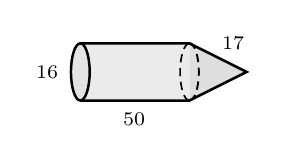
\begin{tikzpicture}[scale=0.66, every node/.style={font=\scriptsize, text=black}]
      % យានអវកាសទី២០៖ ស៊ីឡាំង d=16 (r=8), h1=50 + កោន s=17
      \fill[gray!16] (-1.55,-0.55) rectangle (0.55,0.55);
      \fill[gray!26] (0.55,-0.55) -- (1.65,0) -- (0.55,0.55) -- cycle;
      \fill[gray!22] (-1.55,0) ellipse (0.18 and 0.55);
      \draw[black, line width=0.9pt] (-1.55,0) ellipse (0.18 and 0.55);
      \draw[black, line width=0.9pt] (-1.55,0.55) -- (0.55,0.55) -- (1.65,0) -- (0.55,-0.55) -- (-1.55,-0.55);
      \draw[black, line width=0.7pt, densely dashed] (0.55,-0.55) arc (-90:90:0.18 and 0.55);
      \draw[black, line width=0.6pt, densely dashed] (0.55,0.55) arc (90:270:0.18 and 0.55);
      \node[below=1pt] at (-0.50,-0.55) {$50$};
      \node[left=1pt] at (-1.72,0) {$16$};
      \node[above right=-1pt] at (1.05,0.28) {$17$};
    \end{tikzpicture}
  \end{minipage}
\end{tcolorbox}

\end{document}
